% document style header
\documentclass[a4paper, 12pt]{../../config/homework}

% import default packages
\usepackage{../../config/defpackages}

% import custom math commands
\usepackage{../../config/domath}

% end preamble
\begin{document}

% document title
\noindent
\begin{tabularx}{\textwidth}{>{\centering\arraybackslash}X>{\centering\arraybackslash}X>{\centering\arraybackslash}X}
Calvin \& Alex & MATH 314 Extra Credit & Due 2023 Nov 31\\
\midrule
\end{tabularx}

% homework problems begin
\begin{enumerate}[label=\textbf{Task \arabic*}]
\item Describe the die-rolling example above by defining logical statements \(A\) and \(B\) to set up a proof-by-contradiction argument.
\begin{align*}
\phantom{\therefore}&\,\text{If my friend has a standard 6-sided die, then they will roll a 1, 2, 3, 4, 5, or 6.}\\
\phantom{\therefore}&\,\text{My friend rolled an 8, i.e., they did not roll a 1, 2, 3, 4, 5, or 6.}\\
\therefore & \,\text{My friend did not have a standard 6-sided die.}
\end{align*}

\item Suppose your friend with the die above now pulls out a suspicious-looking coin, and proceeds to flip heads 20 times in a row. Would you believe that the coin is \say{fair}? That is, would you believe that the coin will, in the long run, come up as \say{heads} half of the time? Why or why not?
\\ I would not believe the coin is fair because it flipped heads 20 times in a row.

\item Write the reasoning you used in the previous Task as a three-part argument like the one given above.
\begin{align*}
\phantom{\therefore}&\,\text{If the coin is fair, it will almost certainly come up heads about half the time.}\\
\phantom{\therefore}&\,\text{The coin did not flip heads about half the time.}\\
\therefore&\,\text{The coin is almost certainly not fair.}
\end{align*}

\item How similar do you think the baptismal records that Arbuthnot collected are to the actual birth numbers? What might cause these to be different?
\\ Given the historical influence of the church on every day life it is likely that the baptismal records would be quite similar to actual birth numbers. It seems reasonable to assume that discrepancy in the record is greater attributed to clerical error than that people did not get their kids baptized.

\item What do you notice about the number of boys and the number of girls born each year? Can you think of an explanation for this?
\\ There are more males christened each year than females. It is possible that it was more likely to get sons christened than daughters. Since only sons could enter the priesthood it may not have been as important that daughters be christened.

\pagebreak
\item Do you agree with the mathematics of Arbuthnot's calculation of \({\left(\frac{1}{2}\right)}^{82}\)? If not, how might you explain the different answers?
\\ It seems to be fine. The odds of more males than females being born in a single year is one half, then two years in a row one fourth. It follows that this acts like a coin flip.

\item Arbuthnot concluded that the difference in the number of births of boys and girls could not be due to chance. Do you agree? Why or why not?
\\ Given the data presented it is highly improbable that this is due to chance alone. There remains a considerable effort in demonstrating that the church records are representative of the birth records. This aside, or supposing that they are representative, based on the data presented it is highly improbable that the difference is due to chance alone.

\item Restate and summarize Arbuthnot's explanation using more modern terms.
\\ Arbuthnot argued that males are, and have always been, subject to more dangerous life conditions. Males were the primary hunters of food, work dangerous jobs, etc. This danger exceeds the danger presented to women which, Arbuthnot argues, is primarily diseases. He then claims that to remedy this and ensure more equal pairing of the population God ensures that more males are born.

\item First, write Arbuthnot's main premise as an \say{if \(A\), then aomost-certainly \(B\)} statement. Next, write the contradiction, the \say{not \(B\)} step. Finally, write Arbuthnot's conclusion. Does the structure of his argument in fact match that of the \say{Proof by the Highly Improbably} above?
\\ \(\phantom{\therefore}\) If God is not real then the long term averages of males and females born would almost certainly be equal.
\\ \(\phantom{\therefore}\) The proportion of boys born is consistently larger than the proportion of girls born on each year.
\\ \(\therefore \) God is almost certainly real.
\\ Arbuthnot's argument matches the structure of the Proof by the Highly Improbable.

\item How would you explain Buffon's \say{almost infinite probability} today?
\\ The notion that because we have always observed something to be true, we know it will almost certainly continue to be true.

\item Give another example of something which is \say{physically certain}?
\\ The probability that an object released in open air near the surface of the earth with sufficient mass to make negligible the effect of air resistance, will fall, is \say{physically certain}.

\item Suppose that you know that there was one chance in ten million that you would get in a car crash if you drove to the movie theater tonight. Would that stop you from going? What if there was one chance in ten?
\\ A one in ten million chance of a car accident alone would not stop me from going to the movie theater. My bank account, lack of free time, and inability to eat movie theater popcorn would \textit{but that is besides the point}. A one chance in ten, alone, would heavily deter me from driving my car anywhere.

\item How unlikely would something have to be before you were willing, in practice, to assume that it won't happen? Come up with a specific value and explain why you chose that.
\\ In Ellensburg there is an approximately \(1/2180\) chance of my car getting stolen and I would reasonably say my car will not be stolen. Based on this, for the sake of clarity, I would say anything less likely than a \(1/2000\) chance I would say \say{would never happen}.

\item What value did Buffon settle on as his threshold for moral certainty, and why?
\\ Buffon settled on \(\frac{1}{10000}\) as his threshold for moral certainty. He chose this because this is the probability that a man very near death would die within 24 hours but this man does not experience constant fear thus any probability below this does not contribute to human reasoning and therefore should not contribute to scientific reasoning.

\item Do you think this is a reasonable value? Why or why not?
\\ This value is not reasonable because the reasoning to arrive at the value is not sound. I will suppose the same as Buffon, that at the age of fifty-six an individual has attained \say{full maturity} of reason. If death is inevitable then, by full maturity of reason, it does not make sense to fear death regardless of the probability. Therefore an individual who has truly attained \say{full maturity} of reason would not fear death even if the probability was one in ten. Thus the odds of dying at that age should not be used as the baseline for probability to be near zero for human consideration.

\pagebreak
\item Look up (or possible see your course notes) for a picture fo what the distribution fo these \(\chi^2\) values look like, and draw a picture to demonstrate what Fisher meant in the passage. Is it true that every value of \(P\) corresponds to one value of \(\chi^2\), and that every value of \(\chi^2\) corresponds to one value of \(P\)?
\begin{figure}[h]
    \centering
    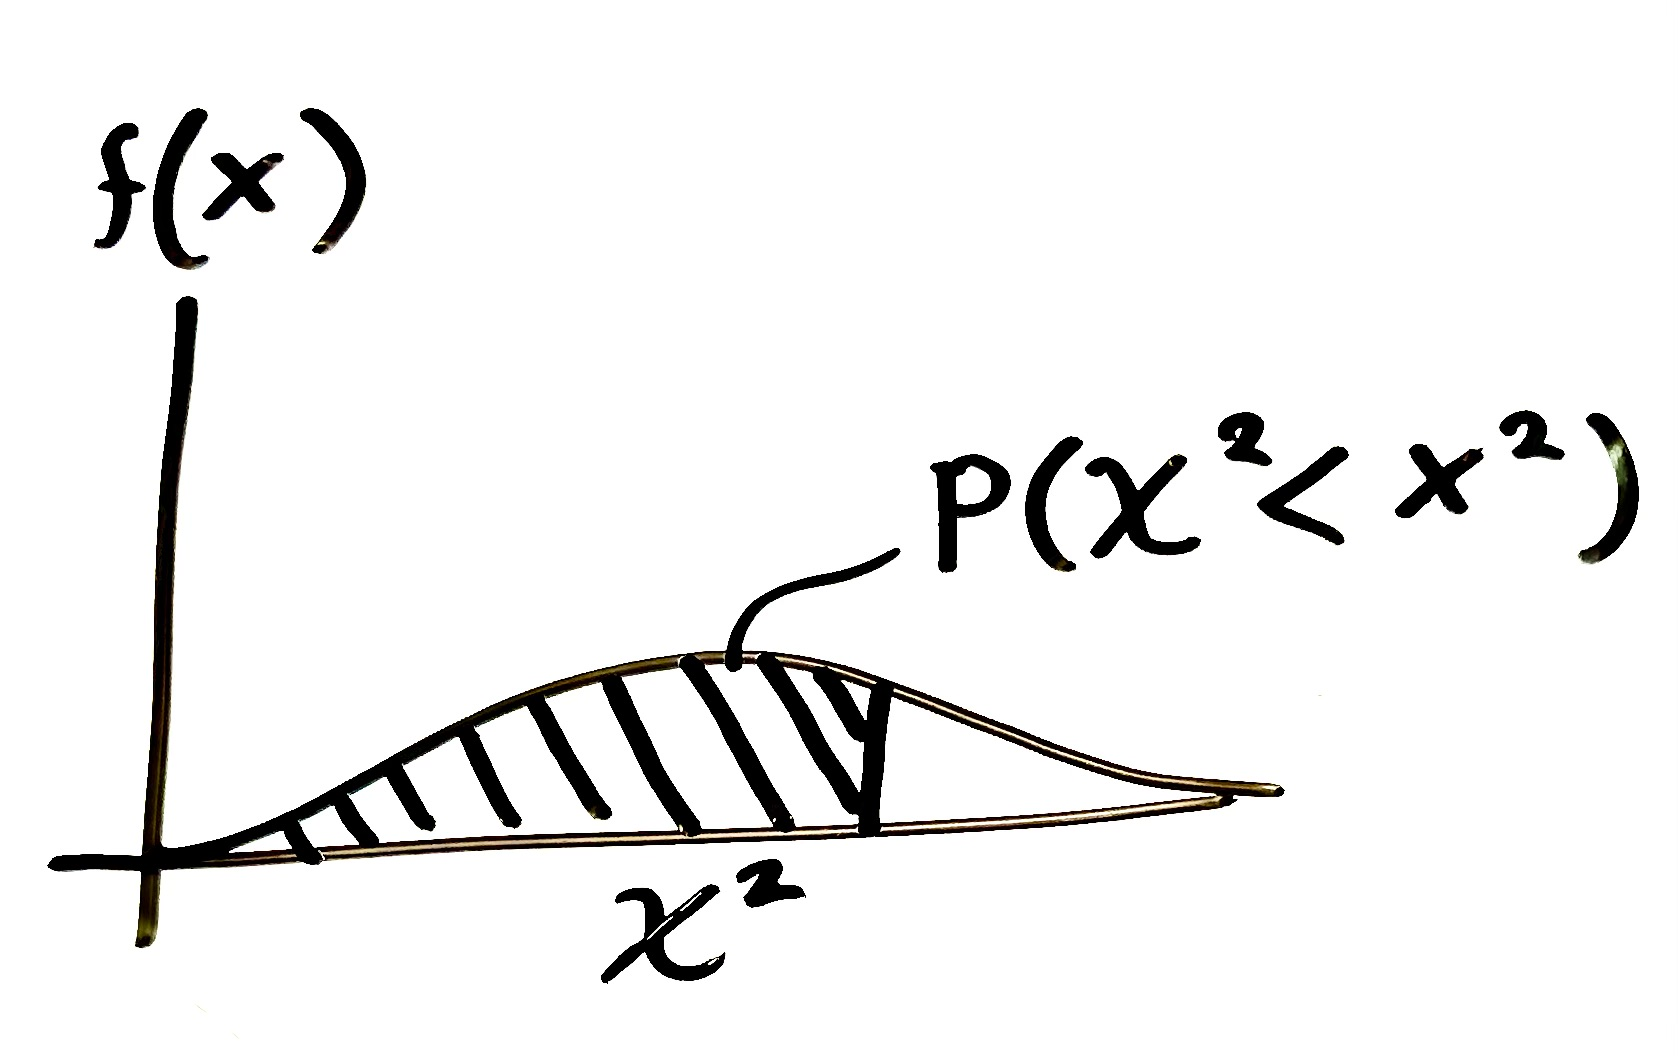
\includegraphics[width=0.6\textwidth]{chi_squared.jpeg}
\end{figure}
The \(\chi^2\) distribution is a function if we consider that \(x\) can only take on positive values. Then Fisher is describing the area under the curve. Shaded is the area \(P(\chi^2 < X^2)\) but in hypothesis testing we consider the area \(P(\chi^2 > X^2)\) to represent the probability that our observation lies beyond the expectation. This is then the p-value.

\item Here Fisher seemed to be arguing for \(P=0.05\) as his threshold value foe whether a deviation from what is expected should be considered \say{significant}. Describe two of the reasons Fisher gave for choosing this value.
\\ Fisher argued this point was significant because we would only be lead astray, by statistics alone, in one of twenty-two trials. Furthermore he states that lowering the standard of significance further may squelch smaller effects.

\item Are these reasons strong enough that you believe we should always choose \(P=0.05\) as a guide to what is significant? Why or why not?
\\ These reasons are not strong enough to justify \(P=0.05\) as a universal standard of significance. A false indication in one of twenty-two trials, by statistics alone, may be fine for some fields research but disastrous in others.

\pagebreak
\item What did Fisher mean when he wrote \say{small effects will still escape notice if the data are insufficiently numerous to bring them out}? Describe a case in which a \say{small effect} might be missed.
\\ Trends in the data that do not reach a \(2\sigma \) significance will not be accepted regardless of how \say{real} they are. A very important historical example in Physics is the discovery of the Higgs Boson. The original detection was only \(2.3\sigma \) which would just barely meet this threshold of significance and did not meet the threshold of significance for physics research which typically requires \(5\sigma \).

\item How is this similar to (or different than) the previous quotation we read from Fisher's work?
\\ This is similar in that Fisher maintained that \(P=0.05\) should be the baseline level of significance, the highest level that we should consider anything to be true. He does however seem to contradict himself in that in his prior statement he stated no \say{no lowering would escape this difficulty}, then proceeds to argue for lowering the standard of significance.

\item Explain Fisher's argument that if a researcher only rejects a hypothesis if \(p < 0.01\) will be \say{mistaken in not more than 1\% of such decisions}.
\\ If a researcher chooses 1\% as their level of significance then they will be wrong less than 1\% of the time. This is because if the hypothesis is correct they will reject it 1\% of the time and if it is incorrect they will never be mistaken because they will nearly always reject it.

\item If a researcher chooses a very high probability for \(p\), say \(p=0.2\), and uses it every time to decide which hypotheses to reject, explain what the negative consequences of this would be.
\\ At this level of significance a researcher may be wrong nearly 20\% of the time. If a hypothesis is correct they may still reject it up to nearly 20\% and if a hypothesis is wrong they may incorrectly accept it. This research allows themselves to be lead astray by statistics alone in one in five experiments.

\pagebreak
\item If a researcher chooses a very low probability for \(p\), say \(p=0.001\), and uses it every time to decide which hypotheses to reject, explain what the negative consequences of this would be.
\\ This researcher will likely reject many true hypothesis but will only accept a false hypothesis one in a thousand times. Thus this researcher will find it very challenge to make statements about reality and will spend their whole time saying \say{we cannot say for certain}.

\item What would you now recommend to a researcher who asks you what value of \(p\) she should choose for her own research?
\\ That is a highly context dependent question. I would ask the researcher about the magnitude of their claims, the potential consequences of accepting a false hypothesis, the amount of data provided, and what other researchers in their field tend to use. For a physicist with access to a myriad of experiments and the desire to make broad claims about the nature of reality one in one million is reasonable. For a scientist concerned with modeling populations whose access to data is limited and the consequences are nearly non-existent for the population modeled one in one hundred is reasonable. The point is that such questions are extremely context dependent and there is not one level of significance that works for everyone asking every question. Arguably the most important level of significance is the one that a majority of researchers in a given field agree on as being significant since researchers who cannot agree on significance will have considerable trouble sharing ideas and conversing in research.

\end{enumerate}
\end{document}
